
\section{Domain Model}

\begin{description}
    \item[User]
        Οποιοσδήποτε χρήστης της εφαρμογής. Με αυτόν τον όρο περιγράφουμε
        οποιοδήποτε άτομο, επιχείρηση ή άλλη οντότητα που αξιοποιεί τις
        υπηρεσίες της εφαρμογής.
    \item[Driver]
        Ένας χρήστης της εφαρμογής ο οποίος οδηγεί κάποιο όχημα.
    \item[Vehicle]
        Ένα όχημα που χρησιμοποιείται για μετακίνηση από κάποιον οδηγό της
        εφαρμογής.
    \item[Rating]
        Η βαθμολογία που δίνει ένας χρήστης σε έναν άλλο χρήστη. Μπορεί να
        περιλαμβάνει σχόλια και εικόνες.
    \item[Report]
        Μια αναφορά που κάνει ένας χρήστης σε έναν άλλο χρήστη για να
        καταγγείλει παράνομη η ανεπιθύμητη δραστηριότητα. Περιλαμβάνει
        κείμενο και έναν λόγο αναφοράς.
    \item[Location]
        Μια γεωγραφική τοποθεσία, περιλαμβάνει διεύθυνση ή συντεταγμένες.
    \item[Route]
        Μια διαδρομή από ένα σημείο Α σε ένα σημείο Β. Μπορεί να περιλαμβάνει
        σημεία στάσης.
    \item[Ride]
        Αντιπροσωπεύει μια συνεπιβίβαση. Ένας οδηγός εκτελώντας μια διαδρομή
        μπορεί να μεταφέρει περισσότερους από έναν επιβάτες οι οποίοι έχουν
        κοινό προορισμό.
    \item[Pickup]
        Αντιπροσωπεύει την παραλαβή ενός επιβάτη από τον οδηγό. Περιλαμβάνει
        σημείο συνάντησης και ώρα.
    \item[Carpooler]
        Ένας χρήστης της εφαρμογής ο οποίος δεν οδηγεί κάποιο όχημα αλλά
        χρησιμοποιεί τις υπηρεσίες της εφαρμογής για να βρει οδηγούς που πάνε
        στο ίδιο μέρος με αυτόν.
    \item[Area]
        Μια περιοχή (πχ ένας δήμος).
    \item[Reward]
        Μία απολαβή είδους κουπονιού-έκπτωσης την οποία μπορεί να εξαργυρώσει
        ο χρήστης.
    \item[Activity]
        Μια δραστηριότητα είναι κάτι το οποίο θέλει να κάνει ο χρήστης σε
        συγκεκριμένο μέρος και ώρα και για το οποίο χρειάζεται μεταφορικό μέσο.
\end{description}

\begin{figure}
    \centering
    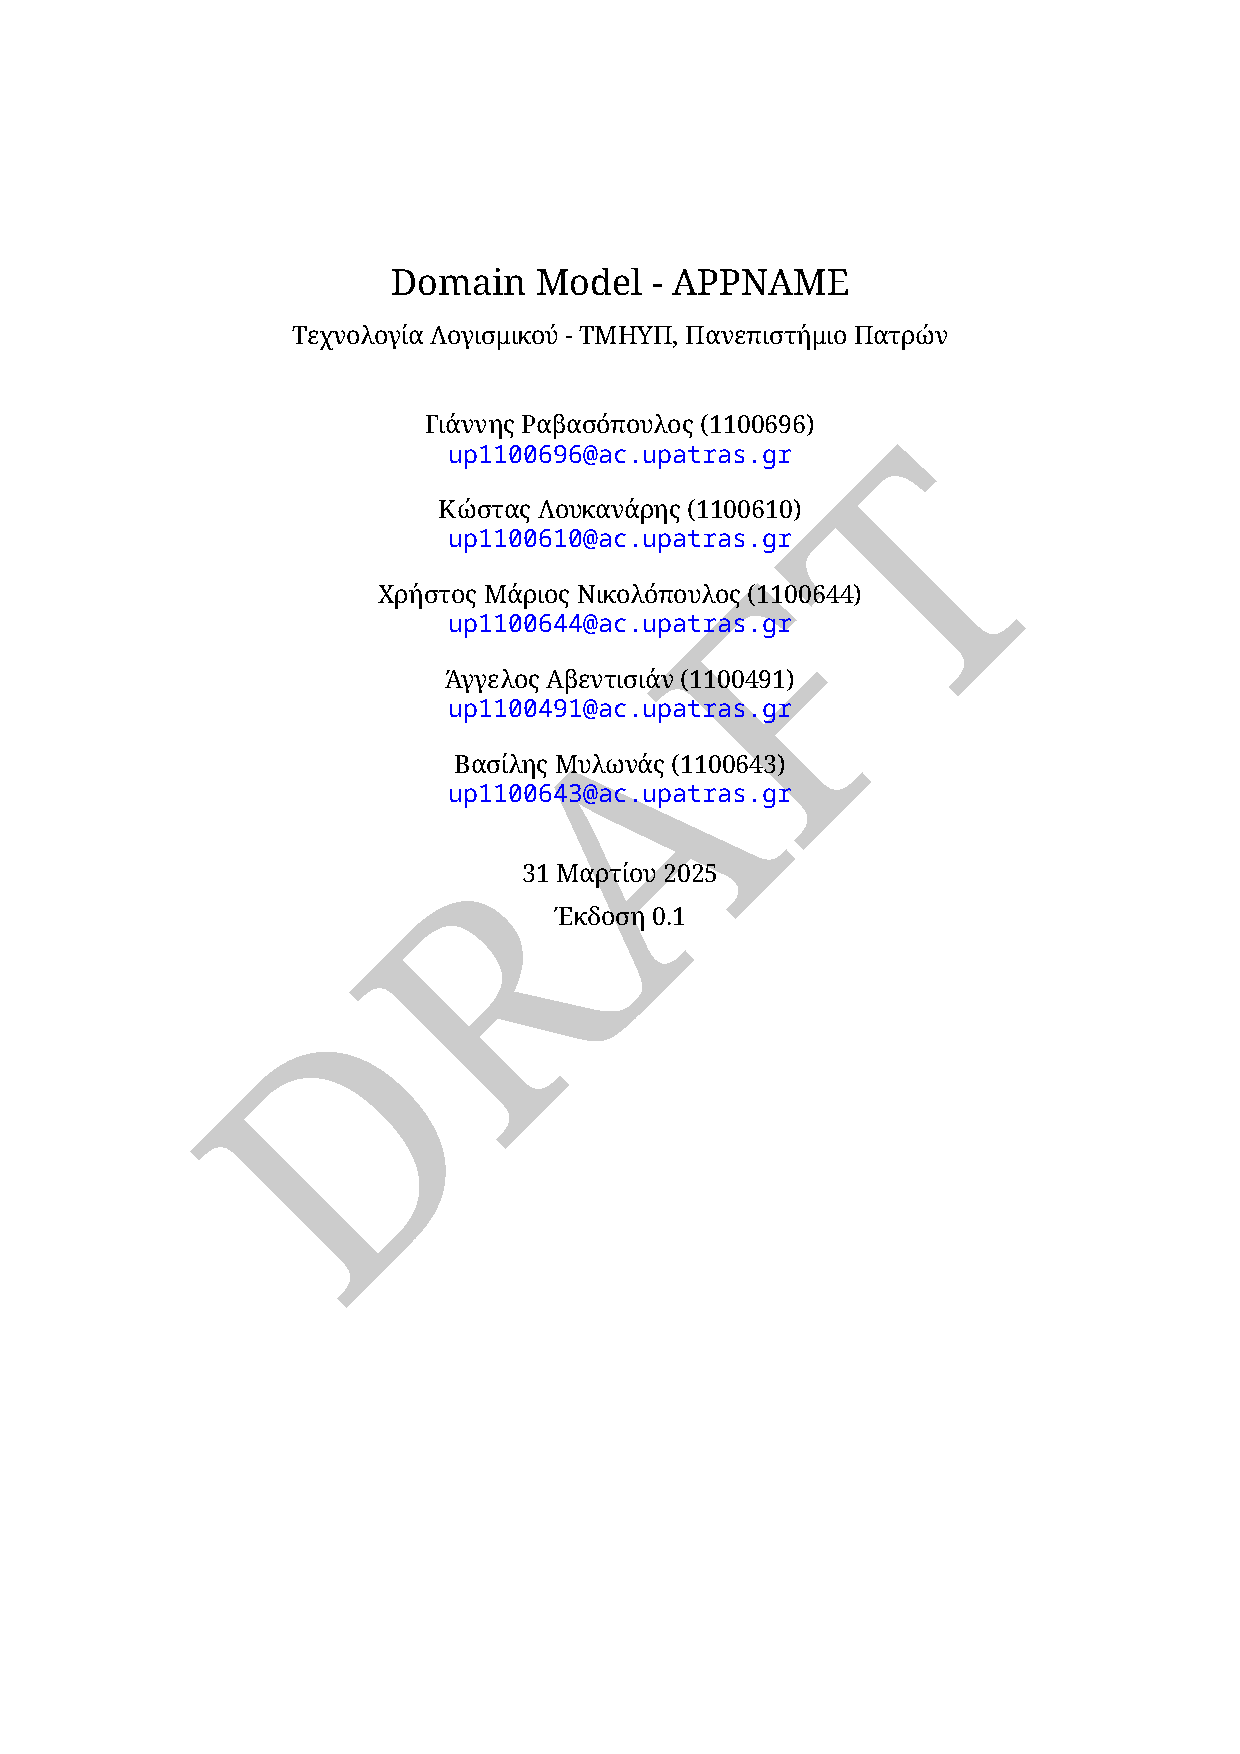
\includegraphics[width=\textwidth]{uml/domain-model}
    \caption{Domain Model}
\end{figure}
